%%%%%%%%%% BEGIN PREAMBLE %%%%%%%%%%
\documentclass[11pt,oneside]{book}
%%%%% PACKAGES %%%%%
\usepackage[top=2.54cm, bottom=2.54cm, left=3cm, right=2cm]{geometry}
\usepackage{graphicx}
\usepackage{lipsum}
\usepackage{amsmath}
\usepackage{amssymb}
\usepackage[font={scriptsize}]{caption}
\usepackage{float} 
\usepackage{changepage}
\usepackage{titlesec}
\usepackage{caption}
\usepackage{minitoc}
\usepackage{empheq}
\usepackage{hyperref}
\usepackage{physics}
\usepackage{xparse}
\usepackage{gensymb}

% fix equation labelling
\numberwithin{equation}{section}

% hyperref parameters
\hypersetup{%
	colorlinks=false,% hyperlinks will be black
	pdfborderstyle={/S/U/W .8}% border style will be underline of width 1pt
}

% minitoc parameters

\setlength{\mtcindent}{24pt}
\renewcommand{\mtcoffset}{0pt}
\mtcsetoffset{minitoc}{0pt}
\setlength{\mtcskipamount}{\bigskipamount}

\setcounter{minitocdepth}{2}  
\renewcommand{\mtcfont}{\small\rmfamily\upshape\mdseries} 
\renewcommand{\mtcSfont}{\small\rmfamily\upshape\bfseries}
% Suppress (sub)section printing in main ToC
\setcounter{tocdepth}{0}

% Change title offset
\titleformat{\chapter}[display]
	{\normalfont\huge\bfseries}{\chaptertitlename\ \thechapter}{20pt}{\Huge}
\titlespacing*{\chapter}{-.5in}{.5pt}{40pt}

%%%%%%%%%% TITLE PAGE %%%%%%%%%
% Create the command for including the title page in the document
\newcommand*{\titleGM}{\begingroup 
	\hbox{ % Horizontal box
		\hspace*{0.2\textwidth} % Whitespace to the left of the title page
		\rule{1pt}{\textheight} % Vertical line
		\hspace*{0.05\textwidth} % Whitespace between the vertical line and title page text
		\parbox[b]{0.75\textwidth}{ % Paragraph box which restricts text to less than the width of the page
			
			{\noindent\Huge\bfseries University of Manchester \\[0.5\baselineskip] Undergraduate \\[0.5\baselineskip]Physics Notes}\\[2\baselineskip] % Title
			{\large \textit{Volume 2}}\\[4\baselineskip] % Tagline or further description
			{\Large \textsc{E. Broadberry, H. Lee Hughes, N. K. Sen}} % Author name
			
			\vspace{0.5\textheight} % Whitespace between the title block and the publisher
	}}
	\endgroup}

%%%%% CUSTOM ENVIRONMENTS %%%%%
% "Examples" environment
\newenvironment{examples}[1][] %DON'T DELETE THESE BRACKETS IT WILL BREAK SHIT
	{\refstepcounter{subsection}
		\par
		\noindent\rule[0.2ex]{\linewidth}{0.1cm}
		\begin{adjustwidth}{1cm}{1cm}
		\medskip
		\noindent \textbf{Examples~\thesubsection #1} \rmfamily}
	{\par
		\end{adjustwidth}
		\noindent\rule[0.2ex]{\linewidth}{0.1cm}
		\medskip}

% "cust_figure" environment
\newenvironment{custfigure}[1][] %DON'T DELETE THESE BRACKETS IT WILL BREAK SHIT
	{\par #1
		\noindent\rule[0.2ex]{\linewidth}{1pt}
		\begin{figure}[H]
		\centering
		\captionsetup{font=small}
		}
	{\end{figure}
		\noindent\rule[0.2ex]{\linewidth}{1pt}
		\medskip}
	
% "dedication" environment
\newenvironment{dedication}[1][]
	{\thispagestyle{empty}		
		\ttfamily
		\begin{center}}          	
	{\end{center}\medskip}        


	
%%%%%%%%%% CUSTOM MACROS %%%%%%%%%%
% Align environment linedrop
\newcommand*{\linedrop}{\\[0.5\baselineskip]}

%(((((((((((((((((((((((( THE FOLLOWING ARE DEPRECIATED BY THE "physics" PACKAGE ))))))))))))))))))))))))

% Dot product 
\newcommand*{\dotp}{\boldsymbol{\cdot}}
% derivative "d"
\newcommand*\diff{\mathop{}\!\mathrm{d}}
\newcommand*\Diff[1]{\mathop{}\!\mathrm{d^#1}}

%(((((((((((((((((((((((( ------------------------------------------------------ ))))))))))))))))))))))))

%%%%% END PREABMLE %%%%%%

\begin{document}
\frontmatter
\thispagestyle{empty} % Removes page numbers
\titleGM % This command includes the title page

% Dedication
\newpage
\begin{dedication}
	This book is dedicated to C. Haunch, L. Heseltine \& L. Rich for putting up with all of our physics bullshit.
\end{dedication}

% Main contents page
\dominitoc
\tableofcontents


\mainmatter
\pagestyle{plain}
% Astrophysical Processes chapter
\chapter{Astrophysical Processes}
\minitoc
\pagebreak
\section{Quantifying radiation}
\subsection{Flux \& intensity}
Recalling from \textit{Introduction to Astrophysics \& Cosmology} we define the energy flux density (or simply flux), $F$ as the power per unit surface area.
%
$$ \diff E = F \diff A \diff t $$
%
Note that flux is dependant on the orientation of the unit surface with respect to the Poynting vector of the radiation field.
 Flux has units of J/s/m$^2$.
 Often it is more useful to use the \emph{monochromatic} energy flux density, $F_\nu$ where
%
\begin{equation}
	\diff E = F_\nu \diff A \diff t \diff \nu
	\label{eq:def_flux}
\end{equation}
%
This gives the energy flux per unit of bandwidth, (frequency interval of radiation) which has units J/s/m$^2$/Hz.
\par 
In order to account for the differing directions of photons, the flux is further generalised by defining the specific monochromatic intensity, $I_\nu$.
 This quantifies the power per unit frequency from a range of directions covering a solid angle element $\diff \Omega$ given by
%
\begin{equation}
	\diff E = I_\nu \diff A dt \diff \nu \diff \Omega.
	\label{eq:def_intensity}
\end{equation}
%
This then has units J/s/m$^2$/Hz/sr.
 Unlike flux, the intensity is constant along the direction of propagation of photons (in free space).
\par
From the respective definitions, we can relate flux and intensity by
%
\begin{align*}
	F_\nu \diff A &= \int \mathbf{I_\nu} \dotp \mathbf{\diff A} \diff \Omega
	\linedrop
	F_\nu \diff A &= \int I_\nu \cos(\theta) \diff A \diff \Omega
	\linedrop
	\therefore F_\nu &= \int I_\nu \cos(\theta) \diff \Omega
\end{align*}
%

\subsubsection{Solid angles: an aside}
The solid angle element $\diff \Omega$ is defined
%
$$ \diff \Omega = sin(\theta) \diff \theta \diff \phi , $$
%
hence when integrated over a complete sphere, $\Omega = 4\pi$~sr.
 This corresponds to the area of a sphere with unit radius.
 Considering the fraction of the total surface area, $A$ of a sphere with radius $R$, we find that
%
\begin{align}
	\frac{A}{4\pi R^2} &= \frac{\Omega}{4\pi}
	\linedrop
	\Omega &= \frac{A}{R^2}.
	\label{eq:solid_angle}
\end{align}
%
As asserted previously, the solid angle corresponds to the area on a sphere with unit radius.
%
\subsubsection{Surface brightness}
Consider an object which a circular region in the sky with radius $\theta_c$.
 We choose to position this object such that it is located at the pole of the coordinate system.
 This is done for convenience such that the setup is rotationally symmetric in $\phi$.
 We can then calculate the flux incident on an aperture.
%
\begin{align*}
	F_\nu &= 2\pi I\nu \int_{0}^{\theta_c}\diff\theta \sin(\theta) \cos(\theta)
	\linedrop
	F_\nu &= \pi I_\nu \sin^2(\theta_c)
\end{align*}
%
For small $\theta_c$, $\sin(\theta_c) \simeq \tan(\theta_c) = R/r$ where $R$ is the object radius and $r$ is the object-aperture distance, hence
%
$$ F_\nu = \pi I_\nu  \left( \frac{R}{r} \right) ^2 \propto \frac{1}{r^2}. $$
%
For an isotropically emitting object (such as a star) the flux can be related to the luminosity (total power generated) by
%
$$ F = \frac{L}{4\pi r^2}. $$
%
%
%
\section{Radiative transfer}
\subsection{Free space}
We want to know how intensity, $I_\nu$ changes along the path of the ray.
 Consider two areas placed parallel to each other with a line length $R$ connecting their centres.
 If the areas are small relative to their separation, then all rays that pass through \emph{both} surfaces are effectively normal to the surfaces.
 From energy conservation,
 %
\begin{align*}
	\diff E_1 &= \diff E_2
	\linedrop
	I_{\nu ,1}\diff A_1 \diff t \diff \nu_1 \diff \Omega_1 &= I_{\nu ,2}\diff A_2 \diff t \diff \nu_2 \diff \Omega_2 ,	
\end{align*}
%
Since, in free space, the frequency remains constant and using equation \ref{eq:solid_angle}:
%
\begin{align*}
		I_{\nu ,1}\diff A_1 \frac{\diff A_2}{R^2} &= I_{\nu ,2}\diff A_1 \frac{\diff A_1}{R^2}
		\linedrop
		I_{\nu ,1} &= I_{\nu ,2}.
\end{align*}
%
Given that the two surfaces have arbitrary size, we can conclude that in general, intensity is conserved along ray paths in free space.
 This is \emph{not} the case for flux.
 Intensity is conserved since it is defined as `per unit solid angle'.
 Hence, for a distance $s$ along the path of a ray,
%
$$ \frac{\diff I_\nu}{\diff s} = 0. $$
%
This is the equation of radiative transfer in free space.
%
%
\subsection{In a medium}
We now need  to consider emission generated along the line of sight as well as absorption by the medium.
 This can be quantified by the equation of radiative transfer in a medium,
%
\begin{equation}
	\frac{\diff I_\nu}{\diff s} = j_\nu - \alpha_\nu I_\nu,
	\label{eq:radiative_transfer}
\end{equation}
%
where $j_\nu$ is the \emph{monochromatic emission coefficient} with units J/s/m$^3$/Hz/sr, and $\alpha_\nu$ is the \emph{monochromatic absorption constant} with units m$^{-1}$.
 It is simple to realise that doubling the intensity passing through a medium would in turn double the intensity absorbed per metre.
 Note that in free space, $j_\nu = 0$ and $\alpha_\nu = 0$.
\par
\subsubsection{Emission coefficient}
From the definition of intensity given by equation \ref{eq:def_intensity}, but changing $\diff E$ to $\delta_E$,
%
\begin{align}
	\frac{\diff \delta_E}{\diff s} &= \frac{\diff I_\nu}{\diff s} \diff A \diff t \diff \nu \diff \Omega
	\linedrop
	\frac{\diff \delta_E}{\diff s} &= j_\nu \diff A \diff t \diff \nu \diff \Omega
	\linedrop
	\therefore \diff \delta_E &= j_\nu \diff V \diff t \diff \nu \diff \Omega.
	\label{eq:emission_coef}
\end{align}
%
From equation \ref{eq:emission_coef} we can see that $j_\nu$ corresponds to the amount of energy radiated per unit volume\footnote{Note that $\diff V = \diff A \diff s$.}, per unit time, per unit solid angle for a frequency interval.
\par 
\subsubsection{Absorption constant}
By using similar treatment for the absorption, we find that
%
\begin{align}
		\frac{\diff \delta_E}{\diff s} &= -\alpha_\nu I_\nu  \diff A \diff t \diff \nu \diff \Omega
		\linedrop
		\frac{\diff \delta_E}{\diff s} &= -\alpha_\nu \delta_E.
		\label{eq:absorption_const}
\end{align}
%
Equation \ref{eq:absorption_const} implies that $\alpha_\nu \diff s$ represents the fraction of energy that disappears from the radiation field after travelling a length $\diff s$ through the medium.
\par  
\subsubsection{Opacity}
Following from the definition in equation \ref{eq:absorption_const}, we now consider a volume of absorbing particles with number density $n$ and absorption cross section $\sigma_\nu$.
 Since each particle obscures an area $\sigma_\nu$, the total area blocked is $n\sigma_\nu\diff V$.
 Also, the fractional area (through which photons flow) that is blocked by absorbers is
$$ n \sigma_\nu \frac{\diff V}{\diff A} = n \diff s \sigma_\nu, $$
hence
% 
\begin{align*}
	\alpha_\nu &= n \sigma_\nu	
	\linedrop
	\alpha_\nu &= \rho \kappa_\nu.
\end{align*}
%
The \emph{opacity coefficient} $\kappa_\nu$ is defined such that $\sigma_\nu \propto \kappa_\nu$. Also, $\kappa_\nu$ has units m$^2$/kg.
\par 
\subsubsection{Optical depth}
Another useful quantity to define is optical depth $\tau_\nu$, which is a re-scaled distance co-ordinate defined by
$$ \diff \tau_\nu \equiv \alpha_\nu \diff s, $$
which provides a more relevan unit to express distance in, rather than metres.
 The total optical depth can then be defined as
$$ \tau_\nu (s) = \int_{s_0}^{s} \alpha_\nu \diff s^\prime. $$
The optical depth becomes particularly useful in the case $j_\nu = 0$.
 In this situation, the equation of radiative transfer (see equation \ref{eq:radiative_transfer}) becomes
$$ \diff I_\nu = - I_\nu \diff \tau_\nu. $$
This differential equation is easy to solve and we find that
%
\begin{equation}
	I_\nu (\tau_\nu) = I_{\nu,0} e^{\tau_\nu}.
\end{equation}
%







 
 
 
\chapter{Complex variables and vector spaces}
\minitoc
\pagebreak
\section{Complex Numbers revision}
\subsection{Basics}
We start with a basic revision of complex numbers.
 Complex numbers were initially introduced to ensure that every polynomial of degree n has n roots. 
 A complex number, $z$, can be expressed in 3 forms:
\begin{enumerate}
	\item $z=x+iy$
	\item $z=R(cos\theta+isin\theta)$
	\item $z=Re^{i\theta}$
\end{enumerate}
In case your memory is that poor, $i$ is the square root of -1.
 Addition of complex numbers is defined as follows $$(x+iy) + (a+ib) = (x+a) + i(y+b) $$
which should be pretty obvious.
 Subtraction is not defined explicitly but by changing $a$ to $-a$ and $b$ to $-b$.
  Multiplication is also defined $$(x+iy)(a+ib) = (ax-by)+i(bx+ay)$$
\subsection{Argand Diagrams}
An argand diagram is a way of representing a complex number on a 2D plane.
 The real component of $z$ is plotted on the x-axis whilst the imaginary component is plotted on the y-axis.
 %
 \begin{minipage}[t]{0.47\linewidth}
 	\begin{figure}[H]
 		\centering
 		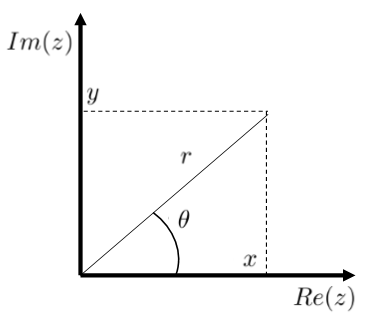
\includegraphics[width=\linewidth]{complex/argand}
 		\captionsetup{font=small} 	
 	\end{figure} 
 \end{minipage}
 \hspace{0.6cm}
%
\begin{minipage}[t]{0.47\linewidth}
	\vspace{1cm}
	We can define the modulus 
	%
	\begin{align*}
	\mid z \mid &= \sqrt{x^2+y^2} \\
	&= (x+iy)(x-iy) \\
	&= z\overline{z}.
	\end{align*}
	%
	In addition to this, $\theta$ is often referred to as the argument.
	 Note that the argument is not unique, you can add $2\pi$ to the argument and obtain the same result, so it's often useful to think of the principal value argument adding the contraint that $\theta$ lies between $0$ and $2\pi$
\end{minipage}
\begin{examples}
	We'll start with a few basic examples to refresh your memory, given $z_1=1+i$ \& $z_2=2+3i$:
	\begin{enumerate}
		\item Find the cube root of $z_1$
		\item Find the modulus and argument of $z_1z_2$
	\end{enumerate}
\textbf{Answers:} 1. $2^{1/6}exp(\frac{\pi}{12})$, $2^{1/6}exp(\frac{3\pi}{4})$, $2^{1/6}exp(\frac{17\pi}{12})$ \hspace{0.5cm}
2. $\mid z\mid = \sqrt{26}$, $arg(z)=1.77$
\end{examples}
\subsection{Mappings}
If we have a complex function, $w=f(z)$, then you can think of this function as a mapping from the domain, the $z$ complex plane, to the co-domain, the $w$ complex plane.
 For example, consider $w=z^2$, what does this mapping look like?
  If we assume $w=u(x,y)+iv(x,y)$ we can see that $u=x^2-y^2$ \& $v=2xy$.

\begin{minipage}[t]{0.47\linewidth}
	\begin{figure}[H]
		\centering
		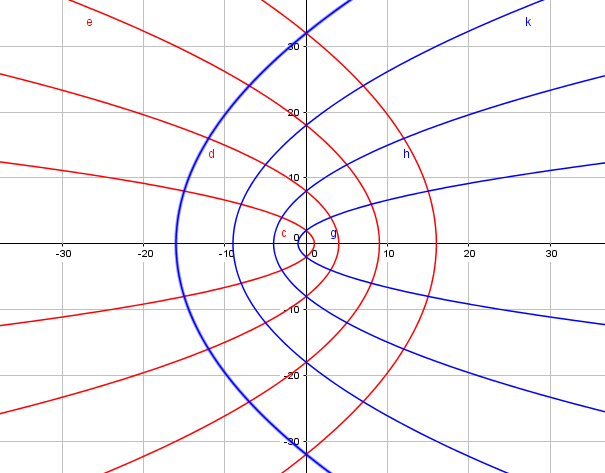
\includegraphics[width=\linewidth]{complex/mapping}
		\captionsetup{font=small} 	
	\end{figure} 
\end{minipage}
\hspace{0.6cm}
%
\begin{minipage}[t]{0.47\linewidth}
	\vspace{0.3cm}
	With a little bit of magic algebra, by setting $x=a$ and $y=b$ we can get 2 relationships.
	\begin{align*}
	\frac{v^2}{4a^2}=a^2-u \\
	\frac{v^2}{4b^2}=u+b^2. \\
	\end{align*}
These 2 equations are plotted on the left for different values of $a$ and $b$. Remembering that $a$ and $b$ are $x$ and $y$ respectively then the red lines are how lines of constant x in the z-plane map into the w-plane.	
\end{minipage}
\include{photonics/intro-photonics}





\end{document}